\documentclass[12pt,fleqn,twocolumn]{article}

\usepackage[english]{babel}
\usepackage[utf8]{inputenc}

\PassOptionsToPackage{hyphens}{url}\usepackage{hyperref}

\usepackage[top=2.5cm, bottom=2.5cm, left=3cm, right=3cm, includeheadfoot]{geometry}

\usepackage{fancyhdr}
\usepackage{graphicx}
\usepackage{float}
\usepackage{changepage}
\usepackage[nottoc, numbib]{tocbibind}
\usepackage{lastpage}
\usepackage{setspace}
\usepackage[bottom]{footmisc}
\usepackage{titling}

\usepackage{amsmath}
\usepackage{amssymb}
\usepackage{nicefrac}
\usepackage{icomma}

\usepackage{csquotes}
\usepackage[backend=biber, style=alphabetic, citestyle=alphabetic, maxcitenames=4, maxbibnames=4, mincitenames=2]{biblatex}

\mathcode`\*=\number\cdot
\newcommand{\numberthis}{\addtocounter{equation}{1}\tag{\theequation}}
\newcommand{\acomm}[1]{\hspace{2.5cm}\text{#1}}
\newcommand{\code}[1]{{\texttt{\small#1}}}

\newcommand{\pro}{\ensuremath{\:\%{}\:}}
\newcommand{\md}{\ensuremath{\text{d}}}
\newcommand{\NN}{\ensuremath{\mathbb N}}
\newcommand{\ZZ}{\ensuremath{\mathbb Z}}
\newcommand{\QQ}{\ensuremath{\mathbb Q}}
\newcommand{\RR}{\ensuremath{\mathbb R}}
\newcommand{\CC}{\ensuremath{\mathbb C}}
\newcommand{\DD}{\ensuremath{\mathbb D}}
\newcommand{\LL}{\ensuremath{\mathbb L}}
\newcommand{\PP}{\ensuremath{\mathbb P}}
\newcommand{\transpose}[1]{\ensuremath{#1^{\textup T}}}

\newcommand{\half}{\ensuremath{\frac{1}{2}}}
\newcommand{\third}{\ensuremath{\frac{1}{3}}}
\newcommand{\fourth}{\ensuremath{\frac{1}{4}}}
\newcommand{\ctp}[1]{\ensuremath{\cdot10^{#1}}}
\newcommand{\reci}{\ensuremath{^{-1}}}

\usepackage[acronym, toc]{glossaries}
\newacronym{dl}{DL}{Deep Learning}
\newacronym{nlp}{NLP}{Natural Language Processing}
\newacronym{dp}{DP}{Differential Privacy}
\newacronym{ml}{ML}{Machine Learning}
\newacronym{dpsgd}{DP-SGD}{Differentially Private Stochastic Gradient Descent}
\newacronym{fl}{FL}{Federated Learning}
\newacronym{dpfa}{DP-FedAvg}{Differentially Private Federated Averaging}
\newacronym{adlm}{AdLM}{Adaptive Laplace Mechanism}

\glsdisablehyper


\addbibresource{references.bib}

\setlength{\droptitle}{-10ex}

\title{Hush-hush Gradients: A Review of Differential Privacy for Deep Learning}

\author{Søren Winkel Holm}
\date{\today}

\pagestyle{fancy}
\fancyhf{}
\lhead{Søren Winkel Holm}
\chead{}
\rhead{Technical University of Denmark}
\lfoot{Differential Privacy for Deep Learning}
\rfoot{Page \thepage{} of \pageref{LastPage}}

\graphicspath{{imgs/}}
\linespread{1.15}

\begin{document}
\setlength{\headheight}{15pt}
\addtolength{\topmargin}{-2.5pt}

\maketitle
\thispagestyle{fancy}
% \tableofcontents

\section*{Introduction}%
\label{sec:Introduction}
The field of \acrfull{dl} is for many subfields moving towards a setup where large multi-purpose foundation models are developed and trained at major companies or research instutitions, and then released for engineers to adapt to specific applications \cite[pp. 3]{bommasani2021oppurt}.
This application of the open-source principle to pre-trained models improves scientific reproduction ability \cite[pp. 3]{hartley2020dtool} and technology accessibility \cite[pp. 139]{bommasani2021oppurt}.
One risk, however, is an adversarial actor exploiting a property of \acrshort{dl} models: 
Parts of training data is generally recoverable from model weights \cite{nasr2019privacy, shokri2017membership}.
This might expose proprietary data or the private data of individuals as exemplified for \acrfull{nlp} language models in Figure \ref{fig:extracting.pdf}.
As large-scale data sets are here to stay \cite{sun2017unreasonable}, algorithmic methods for improving the privacy of foundation models are required.
The methods of \acrfull{dp} are suitable for this task and the relevant concepts, algorithms and problems will here be reviewed.

\begin{figure}[H]
    \centering
        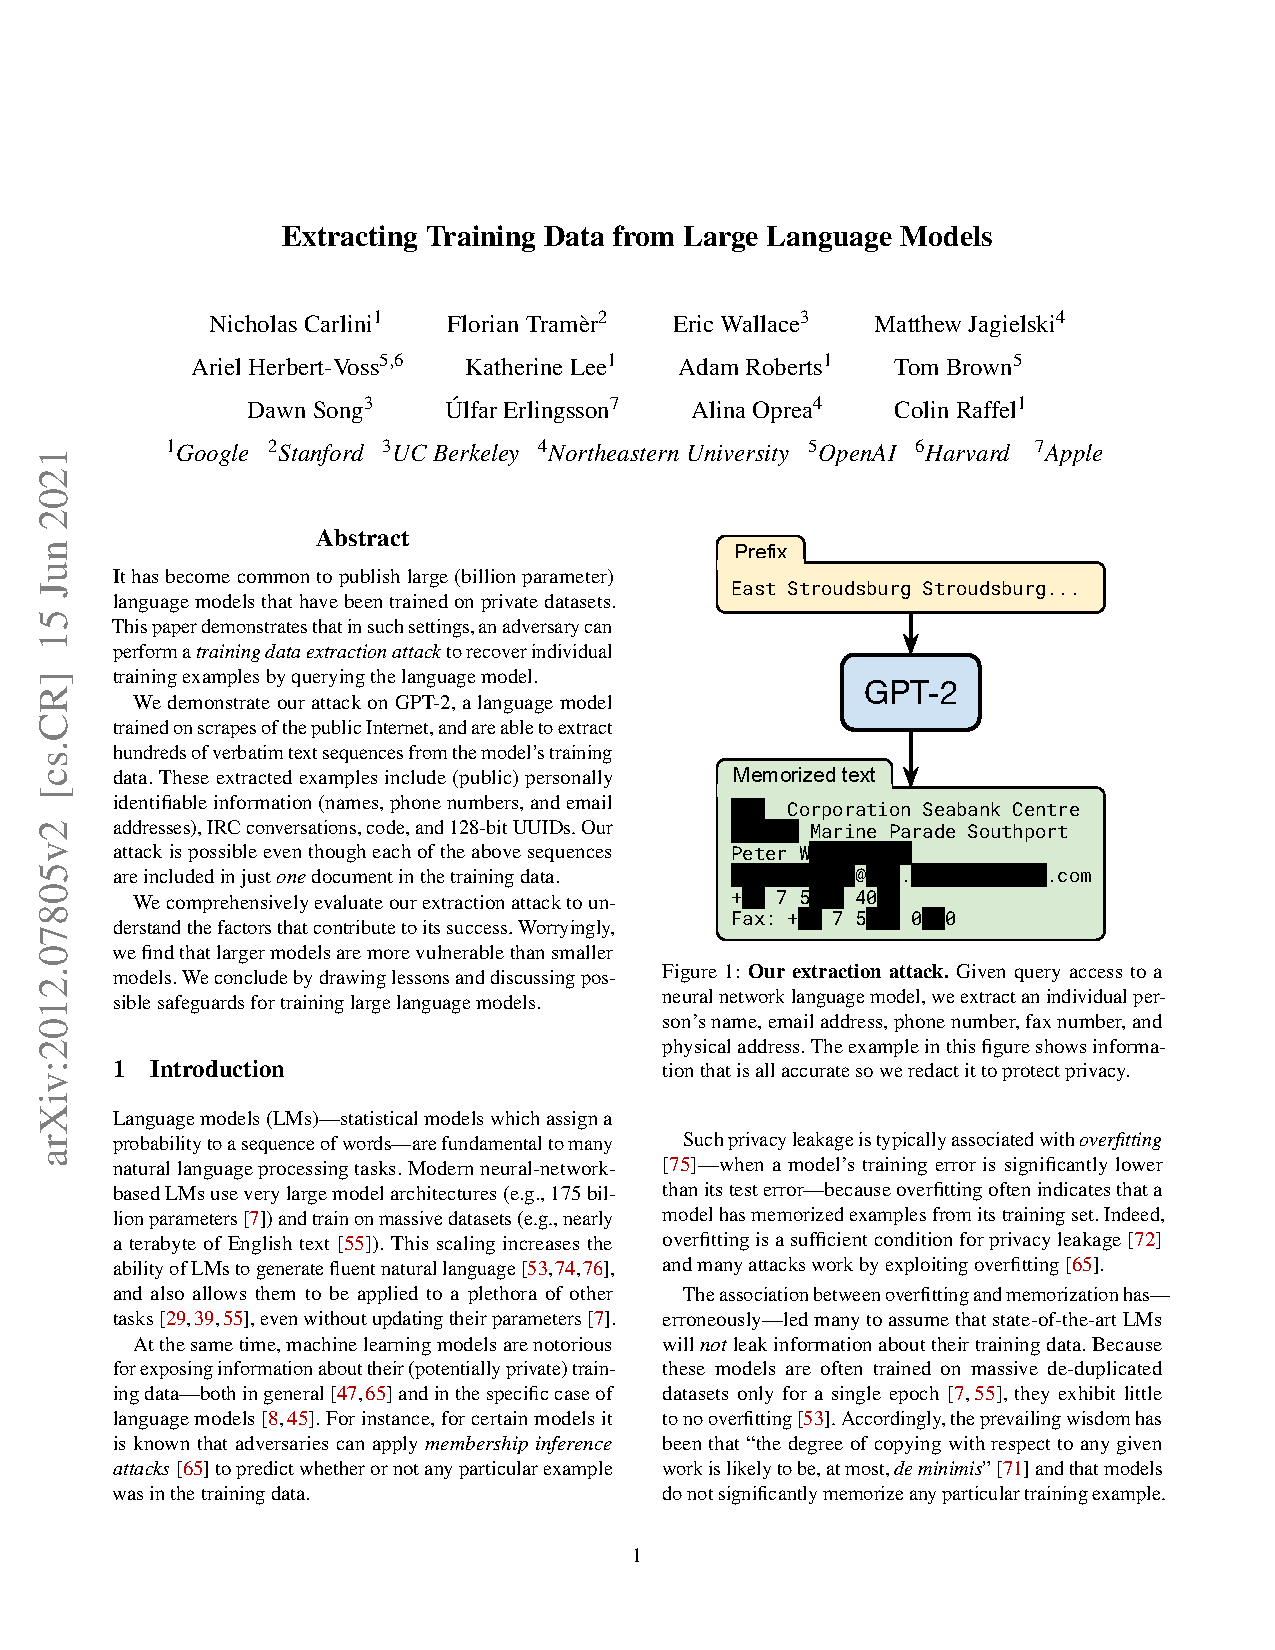
\includegraphics[clip, trim=11.5cm 12cm 2.5cm 8cm, width=.8\linewidth]{extracting.pdf}
        \caption{The private data exposed by GPT-2 found using a simple extraction attack \cite[Fig. 1]{carlini2021extracting} (private data redacted).}
    \label{fig:extracting.pdf}
\end{figure}\noindent

\section*{Fundamental Concepts}%
\label{sec:Fundamental Concepts}
Achieving \acrshort{dp} corresponds to making a promise.
When guaranteeing \acrshort{dp}, you promise hiding information about individuals when publishing quantitative patterns about groups \cite[pp. 5]{dwork2014alg}.
This general problem is historically faced in releases of statistical data analyses by e.g. official organizations \cite{dalenius1977stat, wiki2022diff}.
An algorithm is thus differentially private if a third party observer cannot extract individual information from its' computation.
In this context, a \acrfull{ml} model \(f(x|w)=\hat y \approx y\) trained on a data set \(\mathcal D\) exposes data patterns when either its' parametrization $w$ or predictions $(x, \hat y)$ are released.

Let $\mathcal D_i \in \DD$ be a data set containing the private information of individual $i$ and $\mathcal D_{\hat i} \in \DD$ be identical except excluding this private information.
For most approaches, the goal is to maximise \acrshort{dp} by minimising the impact of individual data on computation.
This goal can be quantified by measures such as the $\ell_1$-sensitivity \cite[pp.31]{dwork2014alg} $\Delta g$ of a numeric statistic $g: \DD \rightarrow \RR^k$,
\begin{equation}
    \Delta g= \operatorname{max}_{i, \hat i \in \DD} ||g(x)-g(y)||_1.
\end{equation}
To lower this, additive noise mechanisms can be used.
For $\Delta g$, this can be achieved by adding Gaussian noise to outputs \cite[D 3.3]{dwork2014alg} 
\begin{equation}\label{eq:gauss}
  f(x)+(Y_1, \ldots, Y_k), Y_i \sim \mathcal N(0, \sigma_{\Delta g}^2)  
\end{equation}
The end goal and golden standard of such \acrshort{dp} mechanisms on random algorithms $\mathcal F(\mathcal D)$ outputting $w \in \operatorname{Im}(\mathcal F)$ with probability $p_{\mathcal F}(w|\mathcal D)$, is to guarantee $(\varepsilon, \delta)$-privacy \cite[Def. 2.4]{dwork2014alg} requiring $\forall S \in \operatorname{Im}(\mathcal F)$ that
\begin{equation}
    P\left(
        \mathcal{F}(\mathcal D_i) \in S
    \right)
    \leq
    \exp(\varepsilon)
    P\left(
        \mathcal{F}(\mathcal D_{\hat i}) \in S
    \right)
    +\delta.
\end{equation}
Thus, for $1-\delta$ of the probability density over algorithmic randomness, it is promised that adding your private data to $\mathcal D$ does not raise your risk of harm by more than $\exp(\varepsilon)$ \cite[pp. 21]{dwork2014alg}.
Often, $\delta=0$, requring the stronger $\varepsilon$-privacy \cite{wiki2022diff}.
For the Gaussian additive noise mechanism \eqref{eq:gauss}, $(\varepsilon, \delta)$-privacy is achieved when $\sigma_{\Delta g}^2=\Delta g \ln(\nicefrac 1 \delta)\varepsilon\reci$ \cite[App. A]{dwork2014alg}.

\acrshort{ml} training procedures are randomized algorithms and as such, simple $(\varepsilon, \delta)$-privacy can be applied directly, though many approaches such as additive noise mechanisms raise the number of samples required to obtain similar performance \cite[pp.221]{dwork2014alg}.
A practical way to integrate the \acrshort{dp} mechanism into \acrshort{dl} training is to modify how the loss gradient estimate $g_t = \nabla \mathcal L(\hat y, y | w_t)$ is used by the optimizer $w_{t+1} = w_t - \eta_t m(g_t)$ \cite{rade2019tensorflow}.
$m$ could add noise or clip the gradient \cite{abadi2016dldp}.

\section*{State of the Art}%
\label{sec:State of The Art}
The foundational application of \acrshort{dp} to \acrshort{dl} was performed at Google by \textcite{abadi2016dldp} in \citeyear{abadi2016dldp} where \acrfull{dpsgd} was presented.
This algorithm modified the gradient estimate of a $B$-sized batch by setting
\begin{align*}
    m(g_t) &= \frac 1 B \Big(
        \sum_{i=0}^B \frac{\mathbf g_t(x_i)}{\operatorname{max}\left(1, || \mathbf g_t(x_i)||_2 C\reci\right)}
    \\ &+ \mathbf e \Big), \mathbf e\sim \mathcal N(0, \sigma^2C^2 \mathbf I),
\end{align*}
where the gradient clipping hyperparameter $C$ and the noise hyperparameter $\sigma$ can be chosen such that is $(\varepsilon, \delta)$-privacy approximately holds for any $\varepsilon, \delta > 0$ \cite[Ch. 3.1]{abadi2016dldp}.
This approximation was achieved using a moment-based \emph{privacy accountant} which tracks the privacy loss of each epoch at the given hyperparameters \cite[Ch. 3.2]{abadi2016dldp}.

When requiring $(8, 10\ctp{-5})$-privacy, the paper found performance drops of $1.3\pro$ for MNIST and $7\pro$ for CIFAR-10 \cite[Chap. 5.3]{abadi2016dldp}, and that computational time was increased by the requirement of single example gradients $\mathbf g_t(x_i)$ especially for convolutional layers \cite[Chap. 4]{abadi2016dldp}.
The clipping performed in $m$ was used for assuring an upper bound on sensitivity from which the correct noise in the Gaussian additive noise mechanism can be used \cite[Chap. 4]{abadi2016dldp}.

\acrshort{dpsgd} remains highly influential and is used as default in leading implementations TensorFlow Privacy \cite{rade2019tensorflow} and PyTorch Opacus \cite{yousef2021opacus}.
The algorithm was swiftly combined with the another main \acrshort{dl} privacy tool, \acrfull{fl} by \textcite{mcmahan2017learningdp} in \citeyear{mcmahan2017learningdp}, producing \acrfull{dpfa} which was used for training a high-performance language model with privacy guarantees \cite[Chap. 3]{mcmahan2017learningdp}.

Using \acrshort{dpsgd} with a privacy accountant limits the number of epochs that are allowed within a given privacy budget $(\varepsilon, \delta)$.
An epoch-agnostic method adding more noise to input features that are deemed less important for learning was presented by \textcite{Phan2017AdaptiveLM} and dubbed \acrfull{adlm}.
Laplace-distributed noise was added to feature relevance scores with hyperparameter $\varepsilon_1$, to layer functions with privacy $\varepsilon_2$, and to the loss function parametrization with hyperparameter $\varepsilon_3$ resulting in $(\varepsilon_1+\varepsilon_2+\varepsilon_3, 0)$-privacy \cite[CHap. III. D]{Phan2017AdaptiveLM}.
\acrshort{adlm} was empirically compared to \acrshort{dpsgd} on MNIST and CIFAR-10, and under fixed $\varepsilon$, \acrshort{dpsgd} generally converged quicker but across all setups, \acrshort{adlm} had the best final accuracy, leveraging the ability to run for unlimited epochs at any $\varepsilon$.
%TODO: HVAD MED DELTA?

A rich literature adding different noise mechanisms to the learning procedure exists.
These approaches balance performance loss, flexibility, privacy guarantees and computational cost and a Google group has attempted to generalize additive mechanisms for \acrshort{dl} \cite{McMahan2018AGA}.
Other recent work is in opposition to this direction arguing that the $(\varepsilon, \delta$)-approach to privacy is best used for single queries from databases, presenting alternative privacy measures created for the cumulative privacy loss induced by many composite computations as is the case for \acrshort{dl} \cite{Yu2019DifferentiallyPM}.

\section*{Open Problems}%
\label{sec:Open Problems}
\begin{itemize}
    \item \emph{What is privacy?} 
      $(\varepsilon, \delta)$-privacy, especially for $\delta=0$, is generally adopted and resulted in a Gödel prize for \textcite{dwork2006cali} but might not easily be communicated to users: ''We are $(1-\delta)\times 100\pro$ sure that your risk of harm is only raised by $\exp{\varepsilon}\times 100\pro$ by giving us your data.''.
      More relevant privacy metrics might communicate some level of absolute chance of extraction.
    \item \emph{How private should data use be?} 
        The choice of the privacy levels represents a negotiation between user and data gatherer.
        Apple has used $2 \le \varepsilon \le 16$, Google has used $2.5$ in a project and the US Census has used $\varepsilon=20$ (all $\delta=0$) \cite{near2022priv}, but in what learning situations are stronger privacy requirements necessary?
    \item  \emph{How to design software that actually keeps privacy promises?}
        It has been highlighted that \acrshort{dpsgd} relies on random batch sampling from the full dataset for a large part of privacy guarantees but is often used with standard data reshuffling in each epoch, resulting in unexpected privacy loss \cite[Chap. III]{Yu2019DifferentiallyPM}.
        In the \acrshort{dl} world where model development is often data-dependant in many complex ways, a software engineering task is present in tracking all use of data and avoiding privacy leakage.
    \item \emph{How to benchmark risk of extraction?}
        If the main \acrshort{dp} worry with use of \acrshort{dl} is user data extraction, a standardized empirical benchmark scoring the privacy risk for e.g. language modelling would be a strong addition to theoretical $\varepsilon$-bounds.
    \item \emph{How to maximize predictive accuracy at a given privacy level?}
        While this broad question underlines all research into \acrshort{dl} and \acrshort{dp}, the literature is not settled on the general approach; should \acrshort{dp} be achieved by noise injection and if so, where in the process?
        Also, as the goal of \acrshort{ml} is to learn a general distribution and not memorize individual examples, \acrshort{dp} should in some sense be a natural consequence of strong \acrshort{ml}.
        \acrshort{dp} should thus perhaps be achieved by architectural, optimizational or data-augmentational improvements seeking to learn more robust and general distributions.
\end{itemize}
\clearpage
\renewcommand*{\bibfont}{\normalfont\footnotesize}
\printbibliography[heading=bibintoc]

\printglossary[type=\acronymtype]

\end{document}
